\documentclass[11pt,a4paper,french]{article}
\usepackage[francais]{babel}
\usepackage[utf8]{inputenc}
\usepackage{a4}
\usepackage{amsmath}
\usepackage{amsfonts}
\usepackage{amssymb}
\usepackage{framed}
\usepackage[amsmath,thmmarks,thref,framed]{ntheorem}
\usepackage[dvips]{graphics}
\usepackage{epsfig}
\usepackage{calc}
\usepackage{tabls}
\usepackage{times}
\usepackage{tabularx}
\usepackage{textcomp}
\usepackage{pst-all}
\usepackage[a4paper]{geometry}

\input{symboles.sty}
\geometry{hmargin=1cm, vmargin=1.5cm}

\title{
DUT d'informatique.\\  
Modélisations Mathématiques.}

\date{}



\begin{document}
\vspace{-2em}
\maketitle
\vspace{-6em}
\begin{center}
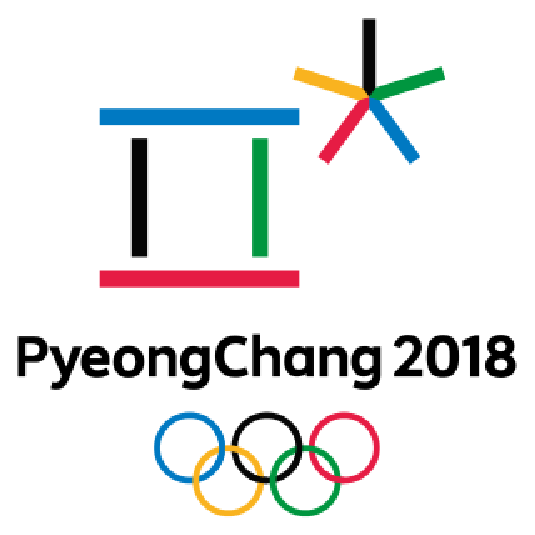
\includegraphics[scale=0.5]{PyeongChang2018}
\end{center}

\vspace{-1em}
\begin{itemize}
\item Prérequis: maximum, minimum, interprétations géométriques de la dérivée, 
\item Objectifs:  étude de fonctions de $R^2$ dans $R$, instruments de mesure pour caractériser les fonctions de  $R^2$ dans $R$.
\end{itemize}


\begin{enumerate}
\item Séance 1: 
\begin{itemize}
\item Compétences:  interprétation de 
tangente, pente, croissance, décroissance, recherche d'extréma, dérivées secondes;
\item Réalisation: exercices classiques de $R$ dans $R$. 
\end{itemize}

\item Séance 2: 

\begin{itemize}
\item Compétences: se familiariser avec des fonctions $R^2$ dans $R$, coupe des lignes de niveau selon un direction;
\item Réalisation: (partiellement en salle machine) générer des fonctions  de 
$R \mapsto R$ avec contraintes sur les dérivées, 
courbes de niveaux,  puis de $R^2 \mapsto R$ croissantes, décroissantes;
dessiner une ligne crête à partir d'une carte IGN; 
proposer des fonctions dont la représentation graphique pourrait ressembler à une piste de ski. 
\end{itemize}

\item Séance 3: 
\begin{itemize}
\item Compétences: calcul et interprétation du gradient (cas particulier du gradient nul), notion de plan tangent et points critiques;
\item Réalisation:  à partir de 2 surfaces données par l'enseignant, analyse de la pente.
\end{itemize}



\item Séance 4: 
\begin{itemize}
\item Compétences: classification des points critiques, 
  matrice hessienne dérivation croisée;
\item Réalisation: creux et bosses (gradient,  et interprétation).
\end{itemize}


\item Séance 5: 
\begin{itemize}
\item Compétences: norme euclidienne;
\item Réalisation: comparaison de gradients, de leur norme, maximisation du gradient et étude de la répartition du gradient sur un maillage.
\end{itemize}

 

\item Séance 5: 
\begin{itemize}
\item Compétences: critique de l'approche (quid lorsque la fonction n'est pas dérivable en un point par exemple);
\item Réalisation:  proposer un modèle de classification des pistes, 
en tenant compte aussi de la longueur de la piste.
\end{itemize}
\end{enumerate}

\end{document}
